% !TEX root = main.tex

% !TEX root = main.tex

\documentclass[14pt,a4paper]{extarticle}
\usepackage[utf8]{inputenc}
\usepackage[T2A]{fontenc}
\usepackage[russian]{babel}
\usepackage{amsmath, amssymb}
\usepackage{geometry}
\usepackage{hyperref}
\usepackage{graphicx}
\usepackage{microtype}
\usepackage{listings}
\usepackage{xcolor}
\usepackage{setspace}
\usepackage{svg}
\usepackage{amsmath}
\usepackage{float}
\usepackage{makecell}
\usepackage{array} % Для вертикального выравнивания m{}
\usepackage{tcolorbox}
\usepackage{tabularx}
\newcolumntype{C}{>{\centering\arraybackslash}X}
\onehalfspacing


\geometry{top=2cm, bottom=2cm, left=1.2cm, right=1cm}
% Определение цветов для классической светлой темы
\definecolor{codegray}{rgb}{0.5,0.5,0.5}
\definecolor{backcolour}{rgb}{0.98,0.98,0.95} % Почти белый фон без желтизны
\definecolor{lightgray}{rgb}{0.95, 0.95, 0.95} % Светло-серый цвет в формате RGB

\lstset{
    language=C++,
    basicstyle=\ttfamily\small,     % Моноширинный шрифт
    keywordstyle=\color{blue},      % Синие ключевые слова
    commentstyle=\color{gray},      % Серые комментарии
    stringstyle=\color{red},        % Красные строки
    numbers=left,                   % Нумерация слева
    numberstyle=\tiny\color{gray},
    stepnumber=1,
    breaklines=true,                % Перенос длинных строк
    frame=none,                   % Рамка вокруг кода
    backgroundcolor=\color{lightgray},
    tabsize=4,
    showstringspaces=false
}

\tcbuselibrary{skins}

\graphicspath{{img/}}

\begin{document}

\begin{center}
    {\Large \textbf{Домашнее задание по курсу \\ "Введение в тензорные компиляторы"}} \\[0.3cm]
    {\large \textbf{Кодогенерация}} \\[1cm]
    
    \textbf{Шелонин Арсений} Б01-411 \\
    \texttt{shelonin.ak@phystech.edu}
\end{center}

\tableofcontents
\newpage

\section{Описание задачи}
B прошлом задании было необходимо перевести код на C в Generic-IR SSA форму и построить CFG.

\paragraph{Исходный код на C} ~\\
\begin{lstlisting}
int function1(int* a, int n) {
    int result = 0;
    for (int i = 0; i < n; ++i) {
        int x = 5;
        for (int j = 0; j < n; ++j) {
            if (j % 2 == 0)
                continue;
            result += 2 * 3 * a[j] * x - i - 2;
        } 
    }

    return result;
}
\end{lstlisting}


\paragraph{SSA IR (optimised)} ~\\
\begin{lstlisting}
int function1(int* a, int n) {
  loop1_preheader:
    result0 = 0;
    i0 = 0;
    loop1_neg_cnd = (i0 >= n);
    br loop1_neg_cnd, exit, loop1_header;

  loop1_header:
    result1 = phi(result0, result5);
    i1 = phi(i0, i2);
    j0 = 1;
    loop2_cnd0 = (j0 < n);
    br loop2_cnd0, loop2_header, loop1_latch;

  loop2_header:
    result2 = phi(result1, result3);
    j1 = phi(j0, j2);
    addr0 = a + j1;
    val0 = *addr0;
    tmp0 = 30 * val0;
    tmp1 = tmp0 - i1;
    tmp2 = tmp1 - 2;
    result3 = result2 + tmp2;
    br loop2_latch;

  loop2_latch:
    result3 = result3;
    j2 = j1 + 2;
    loop2_cnd1 = (j2 < n);
    br loop2_cnd1, loop2_header, loop1_latch;

  loop1_latch:
    result5 = phi(result1, result3);
    i2 = i1 + 1;
    loop1_cnd0 = (i2 < n);
    br loop1_cnd0, loop1_header, exit;

  exit:
    result6 = phi(result0, result5);
    return result6;
}
\end{lstlisting}


\begin{figure}[H]
    \centering
    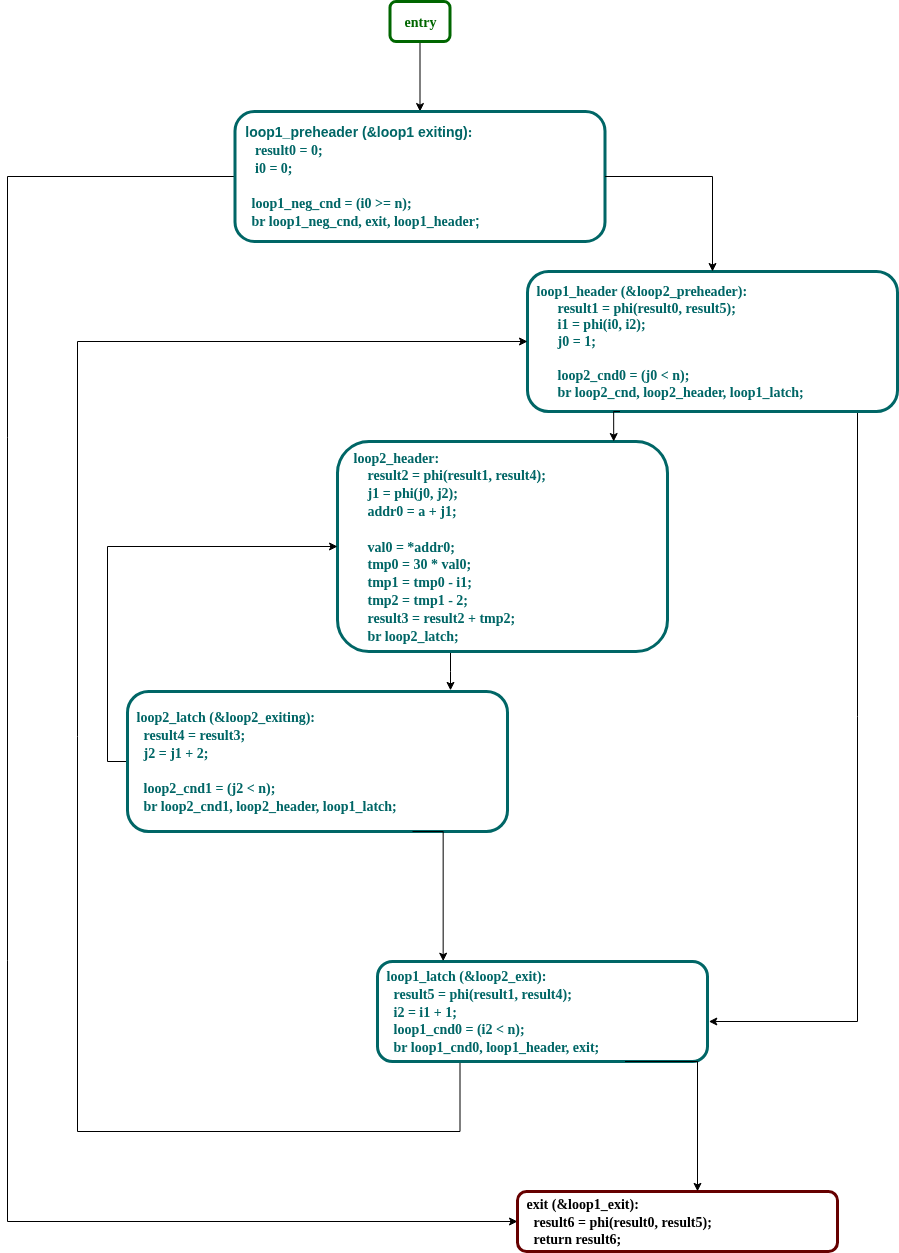
\includegraphics[width=0.99\linewidth]{CFG_SSA_LSR.png}
    \caption{SSA CFG (optimised)}
    \label{fig:SSA_CFG_optimised}
\end{figure}

Сейчас задача состоит в том, чтобы преобразовать Generic-IR код в ассемблер (будет использоваться ассемблер x86-64).

\section{Легализация и выбор}

Архитектура x86-64 требует двухадресного формата инструкций, в то время как Generic-IR имеет трехадресную архитектуру. 

В коде присутствуют многочисленные операции формата \newline
\texttt{addr1 = addr0 + int\_shift0}. Изначально компилятор переводит их в поступательное вычисление адреса с учетом размера типа \texttt{int} и сложения с \texttt{addr0}, но после процесса выбора инструкций происходит матч с инструкций \texttt{lea} и свёртка в неё.

Аналогичным образом сворачивается условный переход.

\begin{table}[h!]
    \small

    \begin{tabularx}{\textwidth}{|p{4.5cm}|c|C|}
        \hline
        \textbf{Операция} & \textbf{Generic IR} & \textbf{x86-64 legalised} \\
        \hline
        Трехадресный код, не поддерживаемый ассемблером & \texttt{tmp3 = tmp1 <op> tmp2} & \texttt{\makecell{mov tmp3, tmp1 \\ <asm\_op> tmp3, tmp2}} \\
        \hline
        Адресная арифметика & \texttt{addr1 = addr0 + int\_shift0} & \texttt{lea addr1, [addr0 + int\_shift0*4]} \\
        \hline
        Условный переход & \texttt{\makecell{cnd0 = (j0 <cnd> j1) \\ br cnd0, bb0, bb1}}  & \texttt{\makecell{cmp j0, j1 \\ jump<cnd> bb0 \\ jmp bb1}} \\
        \hline
    \end{tabularx}
\end{table}

\paragraph{SSA IR (legalised)} ~\\
\begin{lstlisting}
int function1(int* a, int n) {
loop1_preheader:
  mov result0, 0
  mov i0, 0
  cmp i0, n
  jge exit
  jmp loop1_header

loop1_header:
  result1 = phi(result0, result5)
  i1 = phi(i0, i2)
  mov j0, 1
  cmp j0, n
  jl loop2_header
  jmp loop1_latch

loop2_header:
  result2 = phi(result1, result3)
  j1 = phi(j0, j2)
  
  lea addr0, [a + j1*4]
  mov val0, [addr0]
  
  mov tmp0, 30
  imul tmp0, val0
  
  mov tmp1, tmp0
  sub tmp1, i1
  
  mov tmp2, tmp1
  sub tmp2, 2
  
  mov result3, result2
  add result3, tmp2
  
  jmp loop2_latch

loop2_latch:
  mov result3, result3
  
  mov j2, j1
  add j2, 2
  
  cmp j2, n
  jl loop2_header
  jmp loop1_latch

loop1_latch:
  result5 = phi(result1, result3)
  
  mov i2, i1
  add i2, 1
  
  cmp i2, n
  jl loop1_header
  jmp exit

exit:
  result6 = phi(result0, result5)
  ret result6
}
\end{lstlisting}

\section{Разрушение SSA формы}

\paragraph{IR (no SSA)} ~\\
\begin{lstlisting}
int function1(int* a, int n) {
  loop1_preheader:
  mov result0, 0
  mov i0, 0
  
  mov result1, result0
  mov result6, result0
  mov i1, i0
  
  cmp i0, n
  jge exit
  jmp loop1_header

loop1_header:   // result1 <- phi(result0, result5)
                // i1      <- phi(i0, i2)
  mov j0, 1

  mov j1, j0
  mov result2, result1
  mov result5, result1

  cmp j0, n
  jl loop2_header
  jmp loop1_latch

loop2_header:
                // result2 <- phi(result1, result3)
                // j1      <- phi(j0,      j2)
  
  lea addr0, [a + j1*4]
  mov val0, [addr0]
  
  mov tmp0, 30
  imul tmp0, val0
  
  mov tmp1, tmp0
  sub tmp1, i1
  
  mov tmp2, tmp1
  sub tmp2, 2
  
  mov result3, result2
  add result3, tmp2
  
  jmp loop2_latch

loop2_latch:
  mov j2, j1
  add j2, 2
  
  mov result4, result3
  mov j1, j2
  mov result2, result4
  mov result5, result4

  cmp j2, n
  jl loop2_header
  jmp loop1_latch

loop1_latch:
                // result5 <- phi(result1, result4)
  
  mov i2, i1
  add i2, 1
  
  mov i1, i2
  mov result1, result5
  mov result6, result5

  cmp i2, n
  jl loop1_header
  jmp exit

exit:           // result6 <- phi(result0, result5)
  ret result6
}
\end{lstlisting}

\section{Распределение регистров}
Выберем самый нагруженный блок --- loop2\_header --- и распределим в нём регистры линейным подходом.

\begin{lstlisting}
loop2_header:               // a, i1, j1, result2 - already defined
  lea addr0, [a + j1*4]     // def addr0, use a, use j1
  mov val0, [addr0]         // def val0, use addr0
  
  mov tmp0, 30              // def tmp0
  imul tmp0, val0           // use tmp0, use val0, def tmp0
  
  mov tmp1, tmp0            // def tmp1, use tmp0
  sub tmp1, i1              // use tmp1, use i1, def tmp1
  
  mov tmp2, tmp1            // def tmp2, use tmp1
  sub tmp2, 2               // use tmp2, def tmp2
  
  mov result3, result2      // def result3, use result2
  add result3, tmp2         // use result3, use tmp2, def result3
  
  jmp loop2_latch
\end{lstlisting}

\newpage


\begin{figure}[H]
    \centering
    \small
    % Заменяем p на m для вертикального центрирования по середине
    \begin{tabularx}{\textwidth}{@{} m{0.22\textwidth} @{\extracolsep{\fill}} c @{\extracolsep{\fill}} m{0.22\textwidth} @{}}
        
        % ЛЕВЫЙ БЛОК
        \begin{tcolorbox}[
            standard jigsaw, opacityback=0, 
            colframe=black, arc=4mm, 
            width=\linewidth,
            height=6.2cm, 
            valign=center, 
            left=2pt, right=2pt
        ]
            \texttt{\small a: defined \\ i1: defined \\ j1: defined \\ result2: defined \\ addr0: (2, 3) \\ val0: (3, 6) \\ tmp0: (5, 8) \\ tmp1: (8, 9) \\ tmp2: (11, 15) \\ result3: (14, 15)}
        \end{tcolorbox} 
        & 
        % ТАБЛИЦА (Центр)
        \renewcommand{\arraystretch}{1.3}
        % Оборачиваем в таблицу с одним столбцом для выравнивания m
        \begin{tabular}{|p{2cm}|p{2cm}|p{2cm}|}
            \hline
            \textbf{current} & \textbf{live} & \textbf{old} \\ \hline
             addr0  & addr0  &  \\ \hline
               &   &    \\ \hline
               &   &    \\ \hline
               &   &    \\ \hline
               &   &    \\ \hline
            & & \\ \hline
        \end{tabular} 
        & 
        % ПРАВЫЙ БЛОК
        \begin{tcolorbox}[
            standard jigsaw, opacityback=0, 
            colframe=black, arc=4mm, 
            width=\linewidth,
            height=6.2cm, 
            valign=center,
            left=2pt, right=2pt
        ]
            \texttt{\small a: rdi \\ i1: rbx \\ j1: rcx \\ result2: rax \\ addr0: r8 \\ val0: (3, 6) \\ tmp0: (5, 8) \\ tmp1: (8, 9) \\ tmp2: (11, 15) \\ result3: (14, 15)}

        \end{tcolorbox} \\
    \end{tabularx}
\end{figure}



\begin{figure}[H]
    \centering
    \small
    % Заменяем p на m для вертикального центрирования по середине
    \begin{tabularx}{\textwidth}{@{} m{0.22\textwidth} @{\extracolsep{\fill}} c @{\extracolsep{\fill}} m{0.22\textwidth} @{}}
        
        % ЛЕВЫЙ БЛОК
        \begin{tcolorbox}[
            standard jigsaw, opacityback=0, 
            colframe=black, arc=4mm, 
            width=\linewidth,
            height=6.2cm, 
            valign=center, 
            left=2pt, right=2pt
        ]
            \texttt{\small a: defined \\ i1: defined \\ j1: defined \\ result2: defined \\ addr0: (2, 3) \\ val0: (3, 6) \\ tmp0: (5, 8) \\ tmp1: (8, 9) \\ tmp2: (11, 15) \\ result3: (14, 15)}
        \end{tcolorbox} 
        & 
        % ТАБЛИЦА (Центр)
        \renewcommand{\arraystretch}{1.3}
        % Оборачиваем в таблицу с одним столбцом для выравнивания m
        \begin{tabular}{|p{2cm}|p{2cm}|p{2cm}|}
            \hline
            \textbf{current} & \textbf{live} & \textbf{old} \\ \hline
             val0   & val0  & addr0 \\ \hline
                    &       &       \\ \hline
                    &       &       \\ \hline
                    &       &       \\ \hline
                    &       &       \\ \hline
            & & \\ \hline
        \end{tabular} 
        & 
        % ПРАВЫЙ БЛОК
        \begin{tcolorbox}[
            standard jigsaw, opacityback=0, 
            colframe=black, arc=4mm, 
            width=\linewidth,
            height=6.2cm, 
            valign=center,
            left=2pt, right=2pt
        ]
            \texttt{\small a: rdi \\ i1: rbx \\ j1: rcx \\ result2: rax \\ addr0: r8 \\ val0: r8 \\ tmp0: (5, 8) \\ tmp1: (8, 9) \\ tmp2: (11, 15) \\ result3: (14, 15)}

        \end{tcolorbox} \\
    \end{tabularx}
\end{figure}


\begin{figure}[H]
    \centering
    \small
    \begin{tabularx}{\textwidth}{@{} m{0.22\textwidth} @{\extracolsep{\fill}} c @{\extracolsep{\fill}} m{0.22\textwidth} @{}}
        \begin{tcolorbox}[standard jigsaw, opacityback=0, colframe=black, arc=4mm, width=\linewidth, height=6.2cm, valign=center, left=2pt, right=2pt]
            \texttt{\small a: defined \\ i1: defined \\ j1: defined \\ result2: defined \\ addr0: (2, 3) \\ val0: (3, 6) \\ tmp0: (5, 8) \\ tmp1: (8, 9) \\ tmp2: (11, 15) \\ result3: (14, 15)}
        \end{tcolorbox} 
        & 
        \renewcommand{\arraystretch}{1.3}
        \begin{tabular}{|p{2cm}|p{2cm}|p{2cm}|}
            \hline
            \textbf{current} & \textbf{live} & \textbf{old} \\ \hline
             tmp0   & val0  & addr0 \\ \hline
                    & tmp0   &       \\ \hline
                    &       &       \\ \hline
                    &       &       \\ \hline
                    &       &       \\ \hline
            & & \\ \hline
        \end{tabular} 
        & 
        \begin{tcolorbox}[standard jigsaw, opacityback=0, colframe=black, arc=4mm, width=\linewidth, height=6.2cm, valign=center, left=2pt, right=2pt]
            \texttt{\small a: rdi \\ i1: rbx \\ j1: rcx \\ result2: rax \\ addr0: r8 \\ val0: r8 \\ tmp0: r9 \\ tmp1: (8, 9) \\ tmp2: (11, 15) \\ result3: (14, 15)}
        \end{tcolorbox} \\
    \end{tabularx}
\end{figure}


\begin{figure}[H]
    \centering
    \small
    \begin{tabularx}{\textwidth}{@{} m{0.22\textwidth} @{\extracolsep{\fill}} c @{\extracolsep{\fill}} m{0.22\textwidth} @{}}
        \begin{tcolorbox}[standard jigsaw, opacityback=0, colframe=black, arc=4mm, width=\linewidth, height=6.2cm, valign=center, left=2pt, right=2pt]
            \texttt{\small a: defined \\ i1: defined \\ j1: defined \\ result2: defined \\ addr0: (2, 3) \\ val0: (3, 6) \\ tmp0: (5, 8) \\ tmp1: (8, 9) \\ tmp2: (11, 15) \\ result3: (14, 15)}
        \end{tcolorbox} 
        & 
        \renewcommand{\arraystretch}{1.3}
        \begin{tabular}{|p{2cm}|p{2cm}|p{2cm}|}
            \hline
            \textbf{current} & \textbf{live} & \textbf{old} \\ \hline
             tmp1   & tmp1  & addr0 \\ \hline
                    &       & val0  \\ \hline
                    &       & tmp0  \\ \hline
                    &       &       \\ \hline
                    &       &       \\ \hline
            & & \\ \hline
        \end{tabular} 
        & 
        \begin{tcolorbox}[standard jigsaw, opacityback=0, colframe=black, arc=4mm, width=\linewidth, height=6.2cm, valign=center, left=2pt, right=2pt]
            \texttt{\small a: rdi \\ i1: rbx \\ j1: rcx \\ result2: rax \\ addr0: r8 \\ val0: r8 \\ tmp0: r9 \\ tmp1: r8 \\ tmp2: (11, 15) \\ result3: (14, 15)}
        \end{tcolorbox} \\
    \end{tabularx}
\end{figure}


\begin{figure}[H]
    \centering
    \small
    \begin{tabularx}{\textwidth}{@{} m{0.22\textwidth} @{\extracolsep{\fill}} c @{\extracolsep{\fill}} m{0.22\textwidth} @{}}
        \begin{tcolorbox}[standard jigsaw, opacityback=0, colframe=black, arc=4mm, width=\linewidth, height=6.2cm, valign=center, left=2pt, right=2pt]
            \texttt{\small a: defined \\ i1: defined \\ j1: defined \\ result2: defined \\ addr0: (2, 3) \\ val0: (3, 6) \\ tmp0: (5, 8) \\ tmp1: (8, 9) \\ tmp2: (11, 15) \\ result3: (14, 15)}
        \end{tcolorbox} 
        & 
        \renewcommand{\arraystretch}{1.3}
        \begin{tabular}{|p{2cm}|p{2cm}|p{2cm}|}
            \hline
            \textbf{current} & \textbf{live} & \textbf{old} \\ \hline
             tmp2   & tmp2  & addr0 \\ \hline
                    &       & val0  \\ \hline
                    &       & tmp0  \\ \hline
                    &       & tmp1  \\ \hline
                    &       &       \\ \hline
            & & \\ \hline
        \end{tabular} 
        & 
        \begin{tcolorbox}[standard jigsaw, opacityback=0, colframe=black, arc=4mm, width=\linewidth, height=6.2cm, valign=center, left=2pt, right=2pt]
            \texttt{\small a: rdi \\ i1: rbx \\ j1: rcx \\ result2: rax \\ addr0: r8 \\ val0: r8 \\ tmp0: r9 \\ tmp1: r8 \\ tmp2: r8 \\ result3: (14, 15)}
        \end{tcolorbox} \\
    \end{tabularx}
\end{figure}


\begin{figure}[H]
    \centering
    \small
    \begin{tabularx}{\textwidth}{@{} m{0.22\textwidth} @{\extracolsep{\fill}} c @{\extracolsep{\fill}} m{0.22\textwidth} @{}}
        \begin{tcolorbox}[standard jigsaw, opacityback=0, colframe=black, arc=4mm, width=\linewidth, height=6.2cm, valign=center, left=2pt, right=2pt]
            \texttt{\small a: defined \\ i1: defined \\ j1: defined \\ result2: defined \\ addr0: (2, 3) \\ val0: (3, 6) \\ tmp0: (5, 8) \\ tmp1: (8, 9) \\ tmp2: (11, 15) \\ result3: (14, 15)}
        \end{tcolorbox} 
        & 
        \renewcommand{\arraystretch}{1.3}
        \begin{tabular}{|p{2cm}|p{2cm}|p{2cm}|}
            \hline
            \textbf{current}  & \textbf{live} & \textbf{old} \\ \hline
             result3 & tmp2   & addr0 \\ \hline
                    & result3 & val0     \\ \hline
                    &         & tmp0     \\ \hline
                    &         & tmp1     \\ \hline
                    &         & result2  \\ \hline
            & & \\ \hline
        \end{tabular} 
        & 
        \begin{tcolorbox}[standard jigsaw, opacityback=0, colframe=black, arc=4mm, width=\linewidth, height=6.2cm, valign=center, left=2pt, right=2pt]
            \texttt{\small a: rdi \\ i1: rbx \\ j1: rcx \\ result2: rax \\ addr0: r8 \\ val0: r8 \\ tmp0: r9 \\ tmp1: r8 \\ tmp2: r8 \\ result3: rax}
        \end{tcolorbox} \\
    \end{tabularx}
\end{figure}

\newpage

\paragraph{Итоговый ассемблерный код}

Важно обратить внимание на интерфейс вызова функции System V AMD64 ABI. Аргумент 1 передается регистром \texttt{rdi}, аргумент 2 - регистром \texttt{rsi}. Callee-saved регистры - \texttt{rbx, rbp, r12-r15}, то есть мы обязаны сохранить \texttt{rbx}.

\begin{lstlisting}
function1:
push rbx
loop1_preheader:
  mov rax, 0                # result0 = 0
  mov rbx, 0                # i0 = 0
  
  cmp rbx, rsi              # n -> rsi
  jge exit
  jmp loop1_header

loop1_header:
  mov rcx, 1                # j0 = 1

  cmp rcx, rsi              # n -> rsi
  jl loop2_header
  jmp loop1_latch

loop2_header:
  lea r8, [rdi + rcx*4]     # addr0 = a + j1*4
  movsxd r8, dword ptr [r8] # val0 = *addr0
  
  mov r9, 30                # tmp0 = 30
  imul r9, r8               # tmp0 *= val0
  
  mov r8, r9                # tmp1 = tmp0 (tmp1: r8, tmp0: r9)
  sub r8, rbx               # tmp1 -= i1
  
  sub r8, 2                 # tmp2 = tmp1 - 2
  
  add rax, r8               # result3 (rax) += tmp2
  
  jmp loop2_latch

loop2_latch:
  add rcx, 2                # j2 = j1 + 2

  cmp rcx, rsi
  jl loop2_header
  jmp loop1_latch

loop1_latch:
  add rbx, 1                # i2 = i1 + 1

  cmp rbx, rsi
  jl loop1_header
  jmp exit

exit:
  pop rbx
  ret                       # ret rax
\end{lstlisting}


\section{Планирование инструкций блока \texttt{loop2\_header}}

Определим времена раннего и позднего планирования с учётом времени выполнения инструкций:

\hspace{0.5cm}

 \begin{tabular}{|l|l|}
    \hline  
    \textbf{инструкция} & \textbf{время исполнения (такты)} \\ \hline
    lea                 & 1                                 \\ \hline
    mov                 & 1                                 \\ \hline
    imul                & 3                                 \\ \hline
    add                 & 1                                 \\ \hline
    sub                 & 1                                 \\ \hline
\end{tabular} 

\begin{itemize}
    \item Ипользуется \textbf{алгоритм списочного планирования (list sheduling):}
    \begin{enumerate}
        \item Используется два списка:
            \subitem Список готовых: могут начать выполняться прямо сейчас.
            \subitem Список активных --- вызвыаны в предыдущем такте, но всё ещё не готовые
        \item Из списка готовых операций выбираем те, которые будем исполнять на данном такте, и помещаем их в список активных.
        \item Смещаем счётчик такта на единицу.
        \item Если операция из списка активных завершилась — она спланирована.
        \item Если в узле больше нет операций — завершаем алгоритм.
        \item Среди потомков спланированных операций в графе зависимостей ищем такие, аргументы которых уже вычислены, и помещаем в список готовых.
        \item Переходим к п. 1.
    \end{enumerate}
\end{itemize}

\begin{figure}[H]
    \centering
    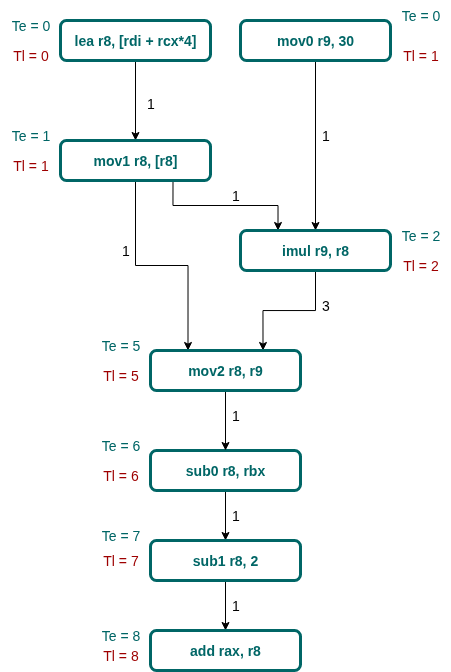
\includegraphics[width=0.5\linewidth]{T_early_late.png}
    \caption{T\_early\_late}
    \label{fig:T_early_late}
\end{figure}


\begin{table}[H]
    \centering
    \small
    \renewcommand{\arraystretch}{1.3} % Увеличение вертикальных отступов для читаемости
    \begin{tabularx}{\textwidth}{|c|c|c|X|X|}
        \hline
        \textbf{такт} & \textbf{m1} & \textbf{m2} & \textbf{готовые} & \textbf{запланированные (активные)} \\
        \hline
        0 & lea & mov0 & lea, mov0 & lea, mov0 \\ \hline
        1 & mov1 & -- & mov1 & mov1 \\ \hline
        2 & imul & -- & imul & imul \\ \hline
        3 & imul & -- & --   & imul \\ \hline
        4 & imul & -- & --   & imul \\ \hline
        5 & mov2 & -- & mov2 & mov2 \\ \hline
        6 & sub0 & -- & sub0 & sub0 \\ \hline
        7 & sub1 & -- & sub1 & sub1 \\ \hline
        8 & add0 & -- & add0 & add0 \\ \hline
    \end{tabularx}
\end{table}

Заметно, как второй АЛУ простаивает практически всё время работы. Это связано с истиными RAW-зависимостями в блоке, что подтверждает практически линейный вид графа выше. 

\end{document}
